\let\negmedspace\undefined
\let\negthickspace\undefined
\documentclass[journal]{IEEEtran}
\usepackage[a5paper, margin=10mm, onecolumn]{geometry}
\usepackage{tfrupee} 
\setlength{\headheight}{1cm} 
\setlength{\headsep}{0mm}     
\usepackage{gvv-book}
\usepackage{gvv}
\usepackage{cite}
\usepackage{amsmath,amssymb,amsfonts,amsthm}
\usepackage{algorithmic}
\usepackage{graphicx}
\usepackage{textcomp}
\usepackage{xcolor}
\usepackage{txfonts}
\usepackage{listings}
\usepackage{enumitem}
\usepackage{mathtools}
\usepackage{gensymb}
\usepackage{comment}
\usepackage[breaklinks=true]{hyperref}
\usepackage{tkz-euclide} 
\usepackage{listings}                                      
\def\inputGnumericTable{}                                 
\usepackage[latin1]{inputenc}                   
\usepackage{color}                                            
\usepackage{array}                                           
\usepackage{longtable}                                       
\usepackage{calc}                                             
\usepackage{multirow}                                         
\usepackage{hhline}                                           
\usepackage{ifthen}                                           
\usepackage{lscape}
\title{5.2.55}
\author{EE25BTECH11052 - Shriyansh Kalpesh Chawda}



\begin{document}
	\maketitle
	\textbf{Question}:\\
	Solve the following system of linear equations.\[
	\frac{2}{x} + \frac{3}{y} = 13 \quad \frac{5}{x} + \frac{4}{y} = -2 \]
	\solution\\
	Let 
	\begin{align}
		u = \frac{1}{x}, \quad v = \frac{1}{y}.
	\end{align}
	The given system becomes
	\begin{align}
		2u + 3v &= 13 \\
		5u + 4v &= -2
	\end{align}
	In matrix form:
	\begin{align}
		\myvec{2 & 3 \\ 5 & 4} \myvec{u \\ v} = \myvec{13 \\ -2}.
	\end{align}
	Let 
	\begin{align}
		A = \myvec{2 & 3 \\ 5 & 4}, \quad \vec{b} = \myvec{13 \\ -2}.
	\end{align}
	We solve using Gauss-Jordan elimination by reducing the augmented matrix $[A|\vec{b}]$ to $[I|\vec{x}]$.
	
	\begin{align}
		\left[\begin{array}{cc|c}
			2 & 3 & 13 \\
			5 & 4 & -2
		\end{array}\right]
		&\xrightarrow{R_1 \rightarrow \frac{1}{2}R_1}
		\left[\begin{array}{cc|c}
			1 & \frac{3}{2} & \frac{13}{2} \\
			5 & 4 & -2
		\end{array}\right] \\
		&\xrightarrow{R_2 \rightarrow R_2 - 5R_1}
		\left[\begin{array}{cc|c}
			1 & \frac{3}{2} & \frac{13}{2} \\
			0 & -\frac{7}{2} & -\frac{69}{2}
		\end{array}\right] \\
		&\xrightarrow{R_2 \rightarrow -\frac{2}{7}R_2}
		\left[\begin{array}{cc|c}
			1 & \frac{3}{2} & \frac{13}{2} \\
			0 & 1 & \frac{69}{7}
		\end{array}\right] \\
		&\xrightarrow{R_1 \rightarrow R_1 - \frac{3}{2}R_2}
		\left[\begin{array}{cc|c}
			1 & 0 & -\frac{58}{7} \\
			0 & 1 & \frac{69}{7}
		\end{array}\right]
	\end{align}
	From the reduced row echelon form, we have the solution:
	\begin{align}
		\myvec{u \\ v} = \myvec{-\frac{58}{7} \\ \frac{69}{7}}
	\end{align}
	Back substituting:
	\begin{align}
		u = \frac{1}{x} = -\frac{58}{7} &\implies x = -\frac{7}{58}, \\
		v = \frac{1}{y} = \frac{69}{7} &\implies y = \frac{7}{69}.
	\end{align}
	Thus, the solution is
	\begin{align}
		\myvec{x \\ y} = \myvec{-\tfrac{7}{58} \\ \tfrac{7}{69}}.
	\end{align}
	\begin{figure}[H]
		\centering
		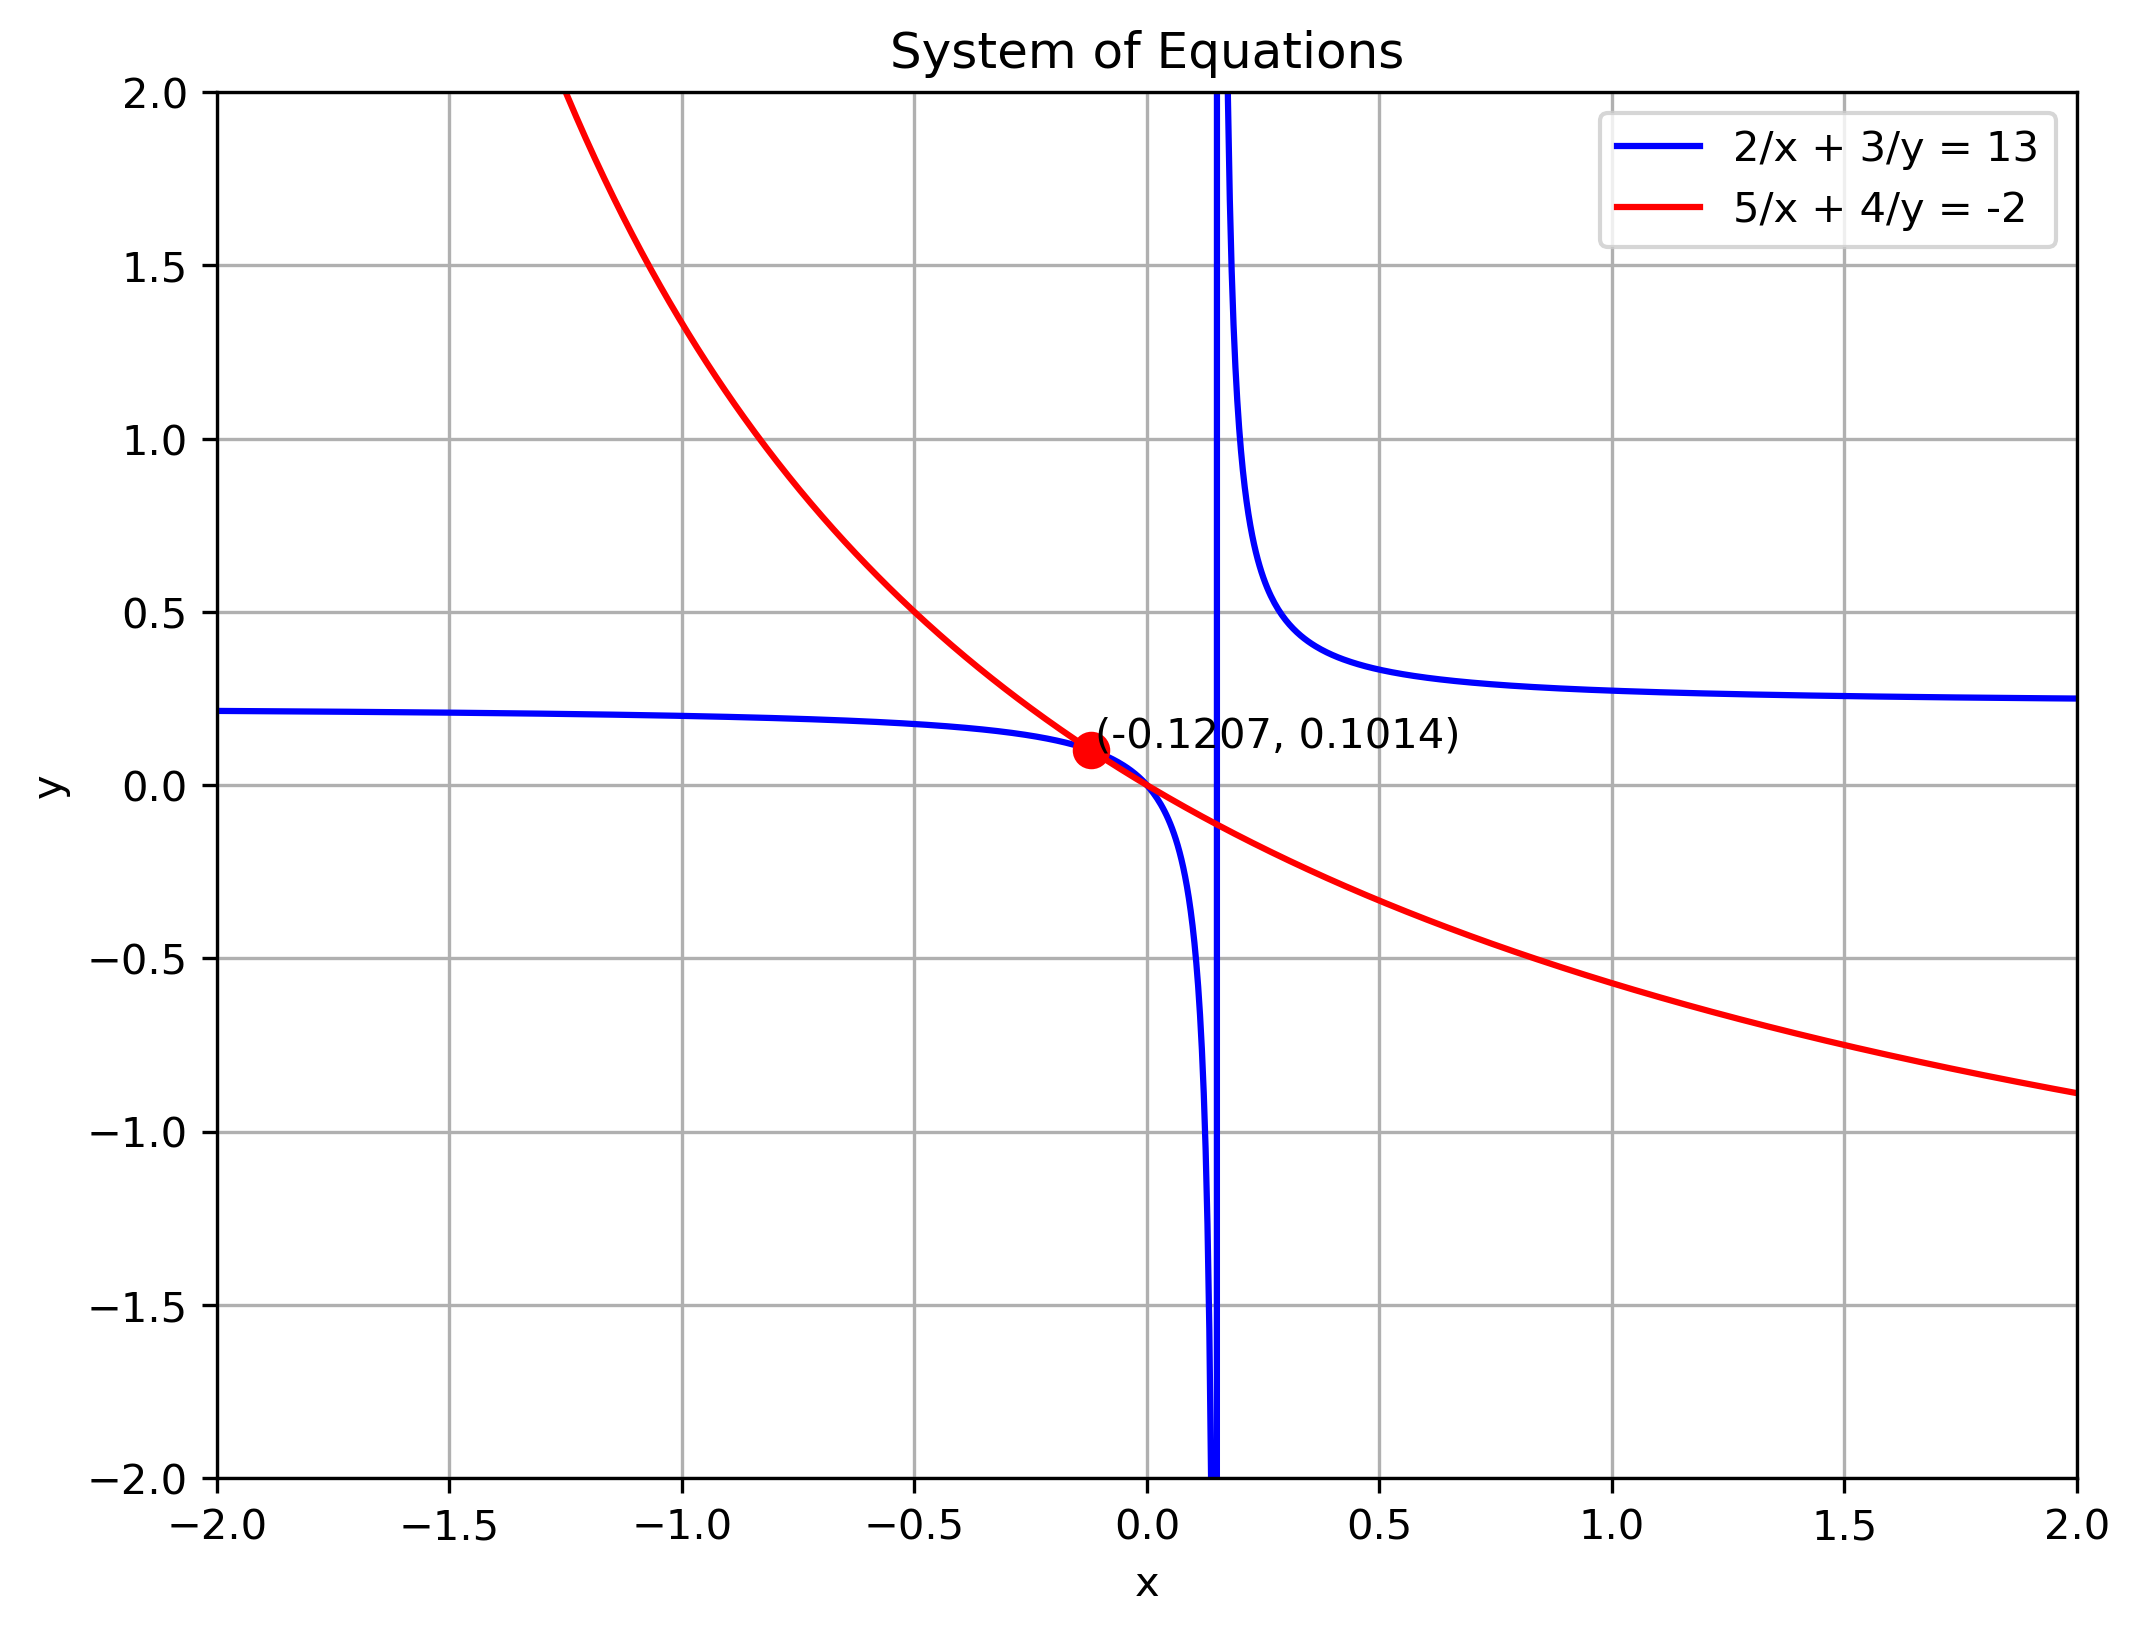
\includegraphics[width=1\linewidth]{figs/equation_plot}
	\end{figure}
	
\end{document}